\chapter{介绍}
	在数据中查找模式的问题是一个基础性问题,并且有很长而成功的历史。例如,Tycho Brahe在16世纪广泛的天文观察是的开普勒发现了天体运动规律,这又提供了经典力学发展的跳板。同样的,原子光谱规律的发现也对量子物理的发展和验证起到了关键的作用。模式识别领域关注于使用计算机算法来自动地发现数据中的规律,并且使用这些规律进行如对不同类别进行分类的一些活动。
	
	思考手写数字的识别例子,如图1.1。每个数字对应$28 \times 28$个像素,可以使用包含784个实数的向量$\mathbf{x}$来表示。目标是去构建一个机器,向量$\mathbf{x}$作为输入,产生数字$0,\dots, 9$作为输出。可以使用手工规则或者启发式来根据笔画形状来区分数字,但是这种方法在实践中会导致增加例外的规则,并且不约而同地给出糟糕的结果。
	
\begin{figure}
	\centering
	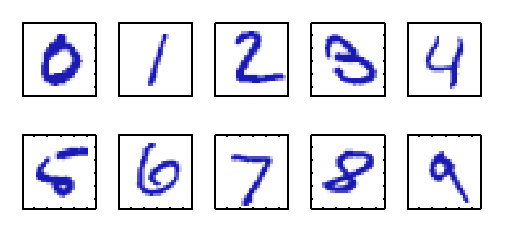
\includegraphics[width=8cm]{Figure1-1.eps}
	\caption{Examples of hand-written digits taken from US zip codes} 
	\label{fig:endb-flow} 
\end{figure}

	更优的结果是采用机器学习方法,这种方法中有一个很大的数字集合N $\{ \mathbf{x_1},$ $ \dots, \mathbf{x_N} \}$ 称为训练集,用来调整得到可适应模型的参数。在训练数据集中的数字分类已经提前给出,通常通过单独手工贴标签来检查他们。我们可以使用目标向量$\mathbf{t}$来表达一个数字的分类,表示对应数字的定义。对于用向量来表示的类别技术会在后面来进行讨论。注意到这里对于每一个数字图像$\mathbf{x}$,使用一个目标向量来表示。
	
	机器学习算法运行的结果可以表示为一个函数$\mathbf{y(x)}$,函数使用一个新的数字图像$\mathbf{x}$作为属兔,产生一个输出向量$\mathbf{y}$,其和目标向量的编码相同。函数$\mathbf{y(x)}$的精确格式在基于训练数据训练阶段时候确定,也被称作学习阶段。当模型确定后,就可以用来确定一个新的的数字图像,包括一个测试数据集。新样本的分类正确性不同于用来训练数据样本的能力称作一般化(generalization)。在实践应用中,输入的各种各样向量使得训练数据可以包含所有可能输入向量的极小部分,并且这也是模式识别的中心目标。
	
	对于大多数的实践应用,原始输入变量都预处理为新空间的变量,是为了希望可以可以很容易地解决模式识别问题。例如,在数字识别问题中,数字的图像通常被转化或者规范化,从而使得每个数字可以在一个固定大小的框中。这可以减少数字类中的变量,因为数字的位置和规模都相同了。这更容易使用子序列模式识别算法在不同类中区别进行区别。这种预处理阶段有时候称为特征提取(feature extraction)。注意到测试数据必须和训练数据一样使用同样的步骤进行预处理。
	
	预处理也会用来提高计算性能。例如,如果目标是在高速视频流的实时人脸检测,计算机必须每秒处理大量的像素,并且直接展示这给一个复杂的模式识别算法或许计算不可行的。代替地,发现有用特征的目标是能计算更快,并且还保留有用的区别信息来使得可以区别人脸和非人脸。这些特征作为模式识别算法的特征。例如,在矩形子区域上的图像强度均值可以非常有效地进行评估,并且一个特征集可以在快速人脸检测上非常有效。因为这些特征的数量比像素点更少,这种预处理表达了降维的一种形式。必须注意到在预处理过程中,因为信息的丢弃,如果这个信息对于处理问题是重要的,那就可以会遭受系统整体精度的痛苦。
	
	训练数据包含的样本是输入向量对于目标向量的应用是监督学习(supervised learning)问题。例如数字识别样本,其中的目标是将每个输入向量赋值为一个有限的离散数字,称为分类问题(classification)。如果期望的输出包含一个或多个连续的变量,这种任务称为回归(regression)。分类问题的一个例子是预测化工生产过程的产率,其中输入包裹关注的反应物,温度和压强。
	
	在其他的模式识别问题中,训练数据包含一个输入向量集$\mathbf{x}$,没有对应任何的目标值。在这种非监督学习(unsupervised learning)问题可能会在数据中发现一组相同样本,称为聚类(clustering),或者在一个输入空间中确定一个数据的分布,称为密度估计(density estimation),或者将高维数据空间投影到两三维,目的是可视化(visualization)。
	
	最后,加强学习(reinforcement learning, Sutton and Barto, 1998)的技术关注的问题是在给定的语境下采取合适的方法去最大化奖励。对于监督学习,学习算法不会输出一个最优的样本,但必须通过实验和错误来发现他们。通常情况下存在一系列的状态和动作,其中学习算法与它的环境交互。在很多例子中,现有的动作不仅仅影响现在的奖励,并且也会对所有的子序列时间步骤产生影响。例如,通过加强学习的技术,神经网络可以学习到下西洋双陆棋达到一个很高的标准(Tesauro,1994)。在这里,网络必须学会将棋盘的一个随机位置作为输入,接着产生一个强的的移动作为输出。这通过将网络与其自己的一个拷贝来对抗来完成,或许会进行百万次。一个主要的挑战是西洋双陆棋会包含很多种移动,只有在游戏结束的时候,在取得胜利的情况下,奖励才得以实现。奖励必须适当地对所有的移动产生贡献,即使一些移动会有好的情况但其他的会差些。这是一种信贷分配(credit assignment)问题。加强学习的一个通常的特征是探索(exploration)和开发(exploitation)之间的权衡,其中探索是系统尝试新的方法来观察他们将会有怎样的效果,而开发系统会使用已知的动作来产生高的奖励。太关注探索或者开发都将会差生较差的结果。加强学习任然是机器学习研究中一个活跃的课题。然而,详细的讨论会超出本书的范围。
	
	尽管每个问题都需要自己的工具和技术,但是很多关键的想法都支撑着所有的这些问题。这章主要的目标是用相关的非形式化方法去介绍介个最重要的的概念和用简单的例子描述他们。在书的后面,我们将会看到这些想法在再出现在更加复杂的模型中,这些模型会适用于真实世界的模式识别中。这章还会包含三个重要工具的介绍,它们会在整本书中都用到,叫做概率理论,决策理论和信息理论。尽管这些听起来像令人畏惧的话题,但是它们事实上是直接的,并且如果将机器学习技术用到实践应用中,清晰地理解它们是必要的。
	
\section{例子:多项式曲线拟合}
	我们通过引入一个简单的回归问题来开始,我们将会用它作为一个运行的例子来贯穿整章来激励一些关键概念。假设我们观察一个真实值输入变量$x$,我们希望使用这个观察值去预测真实值目标变量$t$的值。对于目前的目的,使用合成的方法产生人造样本是具有启发性的,因为当我们进行学习模型比较时候,我们能知道生成数据的精确过程。样本的数据是由在目标值中包含随机噪声的的函数$sin(2 \pi x)$产生的,具体描述见附录A.

	现在假设我们有一个训练集$\mathbf{x} \equiv (x_1, \dots x_N)^T $,包含N个x的观察值,对应的t的观察值表示为$\mathbf{t} \equiv (t_1, \dots t_N)^T $。图1.2展示了包含 N = 10 的训练集的点图。图1.2中的输入数据集$\mathbf{x}$是选择$x_n$的值产生的,对于$n = 1, \dots ,N$,取值范围为[0,1],目标数据集$\mathbf{t}$是通过计算函数数$sin(2 \pi x)$得到的对应值,并对每一个点添加一个低水平的服从高斯分布随机噪声(高斯分布会在1.2.4节介绍)可得到$t_n$。通过这种方式产生数据,我们可以得到很多真实数据集的性质,也就是说这些数据存在潜在的规律,我们希望去学习这种规律,但这种独立的观察值受到随机噪声的干扰。这种平噪声可能从本质上体现随机过程,例如放射性衰变,但是通常是因为变量本省是不可观测的。
	
\begin{figure}
	\parbox{.4\textwidth}{\caption{Plot of a training data set of N = 10 points, shown as blue}}
	\parbox{.5\textwidth}{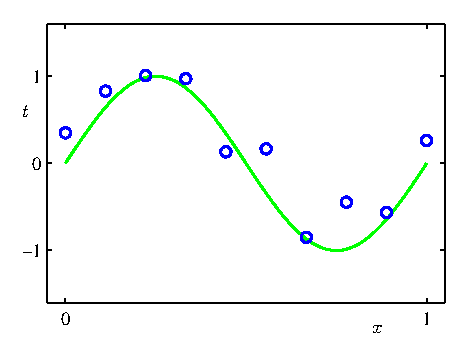
\includegraphics[width=8cm]{Figure1-2.eps}}
\end{figure}

	我们的目标是通过利用训练集,对于一些新的输入变量$\hat{x}$做出预测变量的目标值$\hat{t}$.我们后面可以看到的,这包含隐含地试图找到潜在函数$sin(2 \pi x)$.当我们从有限的数据集中概括时,在本质上是一个棘手的问题。更多的,观察数据集受到噪声的干扰,因此对于一个给定的$\hat{x}$,对应的近似值$\hat{t}$是不确定的。在1.2节中讨论的概率理论提供了一个用精确和定量的方法来表达这种不确定性的框架,在1.5节中讨论的决策理论重现了这种概率的利用,为了根据似然准则做出优化决策。
	
	就目前而言,我们将会非正式地进行和考虑基于曲线拟合的的简单方法,我们使用多项式函数来拟合数据得到形式
	
	\begin{equation}
	y(x,\mathbf{w}) = w_0 + w_1x + w_2x^2 + \dots + w_Mx^M = \sum_{j = 0}^{M}w_jx^j
	\end{equation}
	
	其中M是多项式的阶,$x^j$表示x的j次幂。多项式的系数$w_0, \dots ,w_M$可以使用向量$\mathbf{w}$表示。注意,尽管多项式函数$y(x,\mathbf{w})$是x非线性的函数,但对于w是线性函数。如多项式之类的函数,对于未知参数是线性的,具有重要的性质,称为线性模型,我们将会在3.4节来扩展介绍。
	
	参数的值由对训练数据的多项式拟合确定。这可以表示为通过最小化误差函数(error function),对于任意的值$\mathbf(w)$和训练集数据点,误差函数用来测量函数$y(x,\mathbf{w})$的失配。简单选择被广泛地使用误差函数,通过对每个数据点$x_n$的预测值$y(x,\mathbf{w})$和对应的目标值$t_n$误差平方和,因此我们最小化
	
	\begin{equation}
	E(w) = \frac{1}{2} \sum_{n = 1}^{N}\{ y(x_n,\mathbf{w}) - t_n\}^2
	\end{equation}
	
	其中包含的因子1/2是为了后面计算的方便。我们将会在这个章节的后面讨论使用这个误差函数的原因。现在我们简单地注意到它是一个非负的的等式,当且仅当函数$y(x,\mathbf{w})$精确地通过每一个训练数据点的时候为0。函数平方误差和的几何解析表示为图1.3。
	
	
\begin{figure}
	\parbox{.4\textwidth}{\caption{The error function (1.2) corresponds to (one half of) the sum of the squares of the displacements (shown by the vertical green bars) of each data point from the function $y(x,\mathbf{w})$ } }
	\parbox{.5\textwidth}{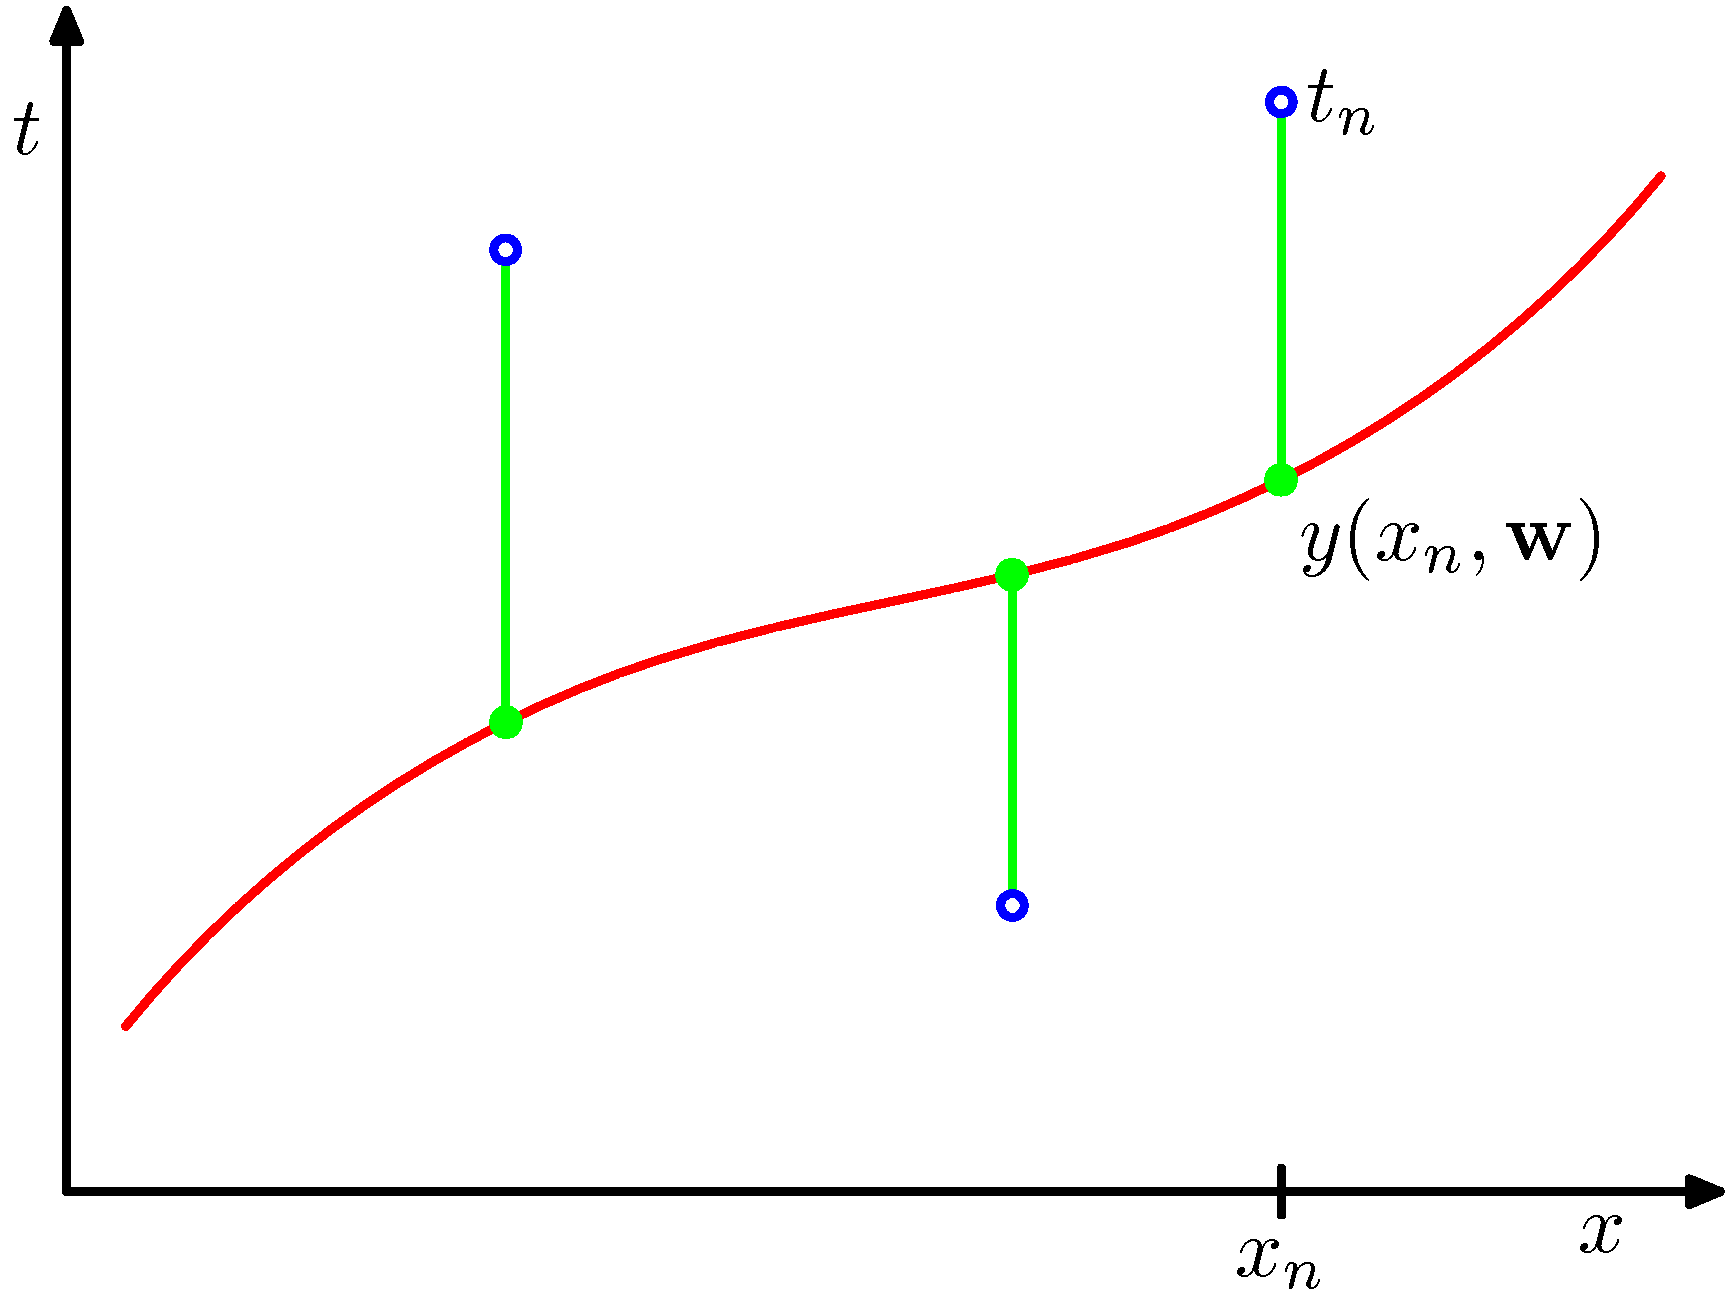
\includegraphics[width=8cm]{Figure1-3.png}}
	\label{fig:endb-flow} 
\end{figure}

	我们可以通过选择$\mathbf{w}$的值来解决曲线拟合问题,其中$E(\mathbf{w})$尽可能小。因为误差函数是参数为$\mathbf{w}$的一个二次函数,它的导数是相对于系数在元素$\mathbf{w}$下是线性的,因此最小化误差函数有唯一的解,可以用紧凑的形式表示为$\mathbf{w}^{\star}$。多项式的结果表示为函数$y(x,\mathbf{w}^{\star})$。
	
	这里存在的问题是如何选择多项式的阶M,我们会看到这会转化为一个重要概念的例子,称为模型对比和模型选择(model comparison or model selection)。在图1.4中,我们展示了对于图1.2中展示的数据集的多项式拟合结果的4个例子,其中多项式的阶数为M = 0,1,3,9。

\begin{figure}[t]
	
	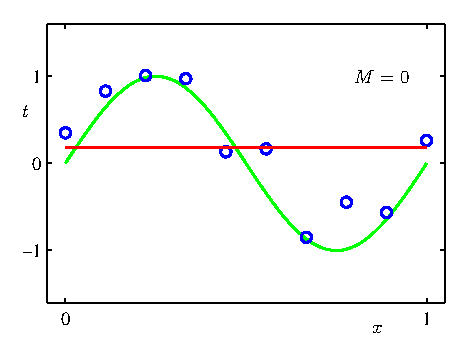
\includegraphics[width=8cm]{Figure1-4a.eps}
	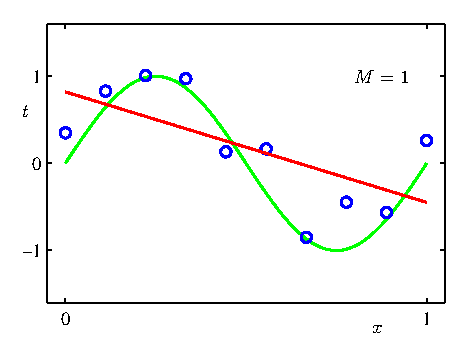
\includegraphics[width=8cm]{Figure1-4b.eps}
	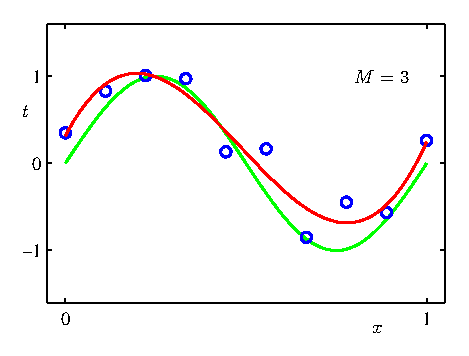
\includegraphics[width=8cm]{Figure1-4c.eps}
	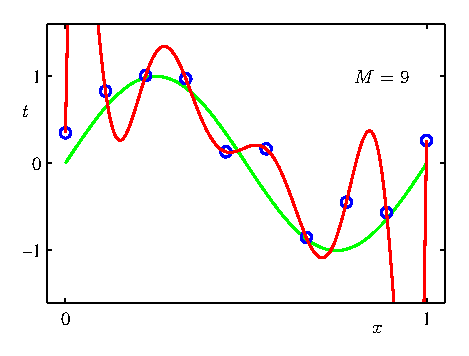
\includegraphics[width=8cm]{Figure1-4d.eps}
	\caption{Plots of polynomials having various orders M, shown as red curves, fitted to the data set shown in
		Figure 1.2. } 
\end{figure}

	我们注意到常量(M = 0)和一次(M = 1)的多项式对于数据得到相当糟糕的拟合,并且对于函数$sin(2 \pi x)$表示也表现很差。如图1.4所示的例子,三次多项式对于函数$sin(2 \pi x)$似乎得到了最好的拟合。当我们采用更高次的多项式(M = 9)时,对于训练数据,我们得到了一个较好的拟合。事实上,多项式精确地通过每个点,并且$E(\mathbf{w}^{\star}) = 0$。反而,拟合曲线较大范围的波动对于函数$sin(2 \pi x)$会得到较差的表示。后面这种行为称为过拟合(over-fitting)。
	
	正如我们前面所描述的,我们的目标是实现对于新数据的精确预测的归纳。我们可以通过考虑单独的测试数据集定量地对这些在M上独立的归纳模型的性能进行观察,其中每个数据集精确地使用和生成训练数据集相同的方法生成的100个数据点,但在目标值中使用新的随机噪声。对于每个选择的M,我们可以对训练数据通过(1.2)式子来评价得到的值$E(\mathbf{w}^{\star})$,并且我们也可以对于测试数据集来评价$E(\mathbf{w}^{\star})$。通常我们使用均方根误差(RMS)来定义更加方便
	
	\begin{equation}
	E_{RMS} = \sqrt{2E(\mathbf{w}^{\star})/N}
	\end{equation}
	
	其中除数M允许我们可以同等地比较不同大小的数据集,并且平方根确保$E_{RMS}$可以和变量t在同一尺度上进行测量。对于不同的M值,训练和测试数据集的REM误差可以在展示在图1.5中。测试数据集是用来测量对于新数据x的观察结果,得到的预测值t的效果如何。我们从图1.5中可以观察到,对于小的M值,会得到相对较大的测试误差。这可以归因于得到的多项式是相当平滑的,并且不能捕获函数$sin(2 \pi x)$的震荡。真如我们所看到的对于图1.4中 M = 3 的例子,M在$3 \leq M \leq 8$范围内时会得到较小的测试误差,并且这也合理地给出了生成函数$sin(2 \pi x)$的表示。

\begin{figure}
	\parbox{.4\textwidth}{\caption{均方根误差的图,定义(1.3),对于不同的M值,用训练集和独立的测试集评估}}
	\parbox{.5\textwidth}{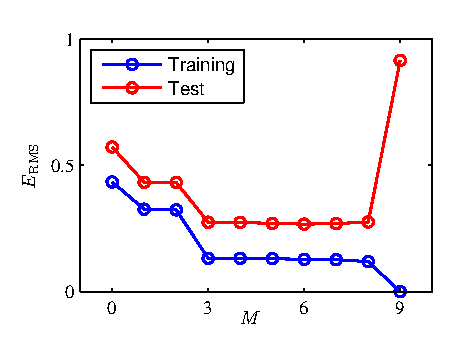
\includegraphics[width=8cm]{Figure1-5.eps}}
	\label{fig:endb-flow} 
\end{figure}

	对于 M = 9,正如我们所预料的,训练集误差为0,因为多项式对应的10个系数包含10个自由度$w_1,\dots,w_9$,所以可以精确地被协调到10个训练数据点。然而,如图1.4所示,测试集误差变得非常大时,对应的函数$y(x, w^{\star})$波动很大。
	
	这似乎是矛盾的,因为一个给定阶数的多项式包含所有低阶的的例子。M = 9 的多项式因此能和 M = 3 的多项式产生一样好的结果。此外,我们或许可以假设对于新数据的最好预测可能是函数来自于函数$sin(2 \pi x)$,其中的数据是由函数生成的(我们后面可以看到这确实是这样的)。我们知道函数$sin(2 \pi x)$的一个幂级数展开包含所有的阶,因此我们期望当我们增加M时,性能会单调地提升。
	
	我们可以通过检验从各种阶数的多项式得到的系数值来得到一些深入的问题,如表1.1所示,我们可以看到,当M增加时,系数的增幅会变得更大。尤其对于M = 9 的多项式,系数完美地在很大的正数和负数之间变换,从而使得多项式函数可以精确地匹配每个数据。但在数据之间,如图1.4中所看到的,函数出现很大的波动。直观地,有很大值M的多项式越平滑,目标值得到的随机噪声越大。
	
	%table1.1
	\begin{table}[b]
		\parbox{.3\textwidth}{\caption{不同阶数的多项式的系数$w^{\star})$,观察当多项式阶数增加时,系数是如何增加的}}
		\parbox{.5\textwidth}{
		\begin{tabular}{r|rrrr}
			& M = 0 & M = 1 & M = 6 & M = 9\\
			\hline
			$w_0^{\star}$ & 0.19 & 0.82 & 0.31 & 0.35 \\
			$w_1^{\star}$ &      & -1.27 & 7.99 & 232.37 \\
			$w_2^{\star}$ &      &       & -25.43 & -5321.83 \\
			$w_3^{\star}$ &  	 & 		 & 17.37 & 48568.31 \\
			$w_4^{\star}$ & 	 & 		 &  	 & -231639.30 \\
			$w_5^{\star}$ & 	 &  	 & 		& 640042.26 \\
			$w_6^{\star}$ & 	 &  	 &  	& -1061800.52 \\
			$w_7^{\star}$ &  	 &  	 &  	& 1042400.18 \\
			$w_8^{\star}$ &  	 &  	 & 		& -557682.99 \\
			$w_9^{\star}$ &  	 & 		 &		&  125201.43
			
		\end{tabular}
	}
	\end{table}
	
	当数据集大小变动时,检验一个给定模型的的行为也是一件有趣的事情,如图1.6所示。我们可以看到,对于一个给定的模型复杂度,当数据集的大小增加时,过拟合问题会变得更小。换句话说,数据集越大时,我们需要的模型就越复杂去拟合数据。一个粗略的启发是,数据点的数量不应该少于模型参数个数的几倍(可能5或者10)。然而,我们可以在第3章中看到,参数的个数并不是衡量模型复杂程度的最合适标准。
	
	\begin{figure}
		
		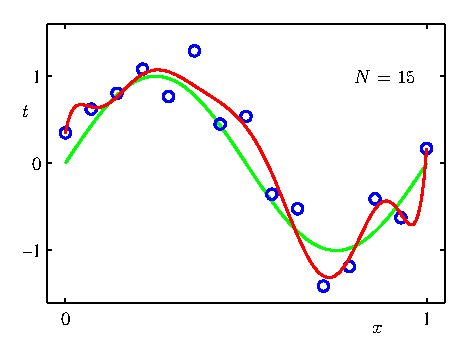
\includegraphics[width=8cm]{Figure1-6a.eps}
		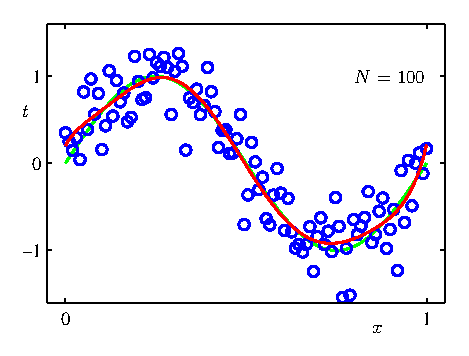
\includegraphics[width=8cm]{Figure1-6b.eps}

		\caption{使用 M =9 的多项式,对于 N = 15(左图) 和 N =100(右图) 的点个数得到的结果,我们可以看到当数据集越大时,过拟合问题越小} 
		\label{fig:endb-flow} 
	\end{figure}
	
	这里也有一些令人很不满意的事,就是必须要根据训练数据集的大小来限制模型参数的个数。这似乎很有道理,根据需要解决的问题的复杂度大小来选择模型的复杂程度。我们可以看到用最小二乘法来找模型参数展现了最大似然估计的一个特殊例子(在1.2.5节中讨论),并且过拟合问题可以理解为最大似然估计的一个通用属性。通过使用贝叶斯方法,过拟合问题可以避免。我们可以发现在模型中利用贝叶斯的方法可以使得参数的个数超过数据点个数。在贝叶斯模型中,真实的参数个数会根据数据集的大小自动调整。
	
	目前,继续用现在的方法和考虑在实践中如何将其应用到有限数据集中是具有指导性意义的,其中我们希望可以使用相对复杂和灵活的模型。通常用来控制过拟合现象的一种技术是正则化(regularization),其中通过添加一个惩罚项到误差函数(1.2)中,可以避免系数达到较大的值。这个惩罚项形式是所有系数的平方和,修改后的误差函数为
	
	\begin{equation}
	\tilde{E}(w) = \frac{1}{2} \sum_{n = 1}^{N}\{ y(x_n,\mathbf{w}) - t_n\}^2 + \frac{\lambda}{2} \parallel \mathbf{w} \parallel^2
	\end{equation}
	
	其中$\parallel \mathbf{w} \parallel^2 \equiv \mathbf{w}^T\mathbf{w} = w_0^2 + w_1^2 + \dots +w_M^2 $,和平方和误差项相比,系数$\lambda$控制正则项的相关重要性。通常系数$w_0$会在正则化中忽略掉,因为将其纳入选择的范围取决于初始变量的选择(Hastie et al., 2001),或者它可以被包含,但是只是正则化它自己的系数(我们将会在5.5.1节详细地讨论这个话题)。式1.4的误差函数可以再次最小化到更接近的形式。这种技术在统计学中称为缩减(shrinkage)方法,因为减少了系数的值。尤其在二次方程正则化中称为岭回归(ridge regression)。在神经网络的环境下,这种方法称为权值衰减(weight decay)。
	
	图1.7展示了9次多项式的拟合结果,数据和之前的一样,但是使用了(1.4)式给出的正则化的误差函数。我们可以看到,对于$\ln \lambda = -18$,过拟合已经被压制了,我们可以得到一个更加接近函数$sin(2 \pi x)$的表达式。然而,当我们使用较大的$\lambda$值时,我们会得到比较差的拟合,如图1.7所示,对于$\ln \lambda = 0$。拟合的多项式对应的系数在表1.2中给出,表明正则化对减少系数的数量级具有所希望的效果。
	
	\begin{figure}
		
		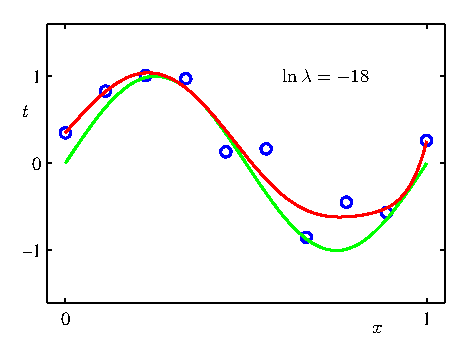
\includegraphics[width=8cm]{Figure1-7a.eps}
		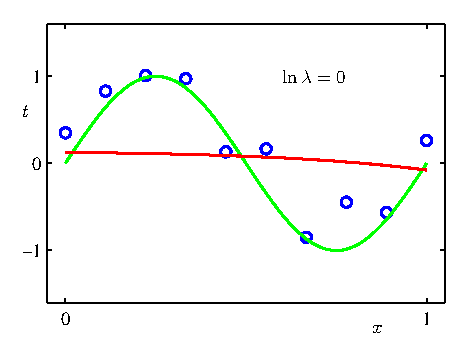
\includegraphics[width=8cm]{Figure1-7b.eps}
		
		\caption{对在图1.2中展示的数据集用M=9的多项式拟合,使用(1.4)的正则化误差函数,两个正则化参数$\lambda$对应$\lambda = -18$ 和$\lambda = 0$} 
		\label{fig:endb-flow} 
	\end{figure}
	
	%table1.2
	\begin{table}[b]
		\parbox{.4\textwidth}{\caption{对于M = 9的多项式,不同的正则化参数$\lambda$值的系数$w^{\star}$。注意当$\ln \lambda = -\inf$时对应的模型没有正则项,即对应图1.4的右下角的图,我们看到,当$\lambda$的值增加时,系数的数量级变得更小}}
		\parbox{.5\textwidth}{
			\begin{tabular}{r|rrr}
				& $\ln \lambda = -\inf$ & $\ln \lambda = -18$ & $\ln \lambda = 0$ \\
				\hline
				$w_0^{\star}$ & 0.35 & 0.35 & 0.13\\
				$w_1^{\star}$ & 232.37 & 4.74 & -0.05 \\
				$w_2^{\star}$ & -5321.83 & -0.77 & -0.06 \\
				$w_3^{\star}$ & 48568.31 & -31.97 & -0.05 \\
				$w_4^{\star}$ & -231639.30 & -3.89 & -0.03 \\
				$w_5^{\star}$ & 640042.26 & 55.28 & -0.02\\
				$w_6^{\star}$ & -1061800.52 & 41.32 & -0.01 \\
				$w_7^{\star}$ & 1042400.18 & -45.95 & -0.00 \\
				$w_8^{\star}$ & -557682.99 & -91.53 & 0.00 \\
				$w_9^{\star}$ & 125201.43 & 72.68 & 0.01
			\end{tabular}
		}
	\end{table}
	
	如图1.8所示,随着$\lambda$的变化,正则项对生成误差的影响可以通过RMS误差的点图看出。我们可以看出$\lambda$控制模型复杂度的效果和确定过拟合的程度。
	
	\begin{figure}[t]
		\parbox{.4\textwidth}{\caption{对于M = 9的多项式,随着$\ln \lambda$的变化的均方根误差图}}
		\parbox{.5\textwidth}{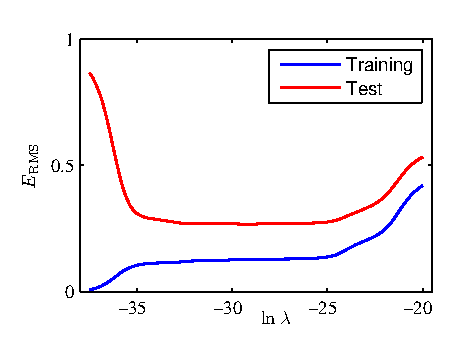
\includegraphics[width=8cm]{Figure1-8.eps}}
	\end{figure}
	
	模型复杂度问题是一个重要的问题,我们会在后面的1.3节详细介绍。这里我们简单了解一下,如果我们用最小化误差函数这种方法来解决一个实际应用,对于模型复杂度,我们必须找到一种方法去确定一个合适的值。上面的结果建议一种简单的方法来实现,通过合适地利用数据,把数据分为一个训练集和确认集(validation set),训练集用来确定系数$\mathbf{w}$,确认集也称为保留集(hold-out set),用来最优化模型复杂度(M或者 $\lambda$)。然而,在很多例子用,这种方法被认为是太浪费训练数据了,我们必须找到更复杂的方法。
	
	目前我们讨论的多项式曲线拟合很依赖直觉。我们现在寻找一种一种更具原理性的方法来解决问题,在模式识别中,通过将问题转化为概率论来解决。上面讨论的内容几乎是这本书中所有的子内容,为我们打下了基础,也为我们介绍多项式曲线拟合的概念内容提供了重要的视角,并且也允许我们扩展到更复杂的情况。
	
\section{概率论}
	在模式识别中一个重要的概念是不确定性。不确定性出现在测量的噪声中,也存在于有限的数据集中。概率论为定不确定性的定量和操作提供了一系列的框架,并形成了模式识别的核心基础。当概率论与决策理论结合起来时,我们可以对于给定的所有信息,作出最优的决策,即使提供的信息不完整或者具有二义性。
	
	我们将会通过考虑一个简单的例子来介绍概率论的基本概念。想象我们有两个箱子,一个是红色,一个是蓝色,在红色的箱子中有2个苹果和6个橘子,在绿色的箱子中有3个苹果和一个橘子,如图1.9所示。现在我们假设随机地挑选一个箱子,从箱子中随机地选出一个水果,观察水果的种类,然后从原来的箱子中移除。我们可以想象重复这个过程很多次。让我们来假设这样做,40\%的次数选红箱子,60\%的次数选蓝箱子,当我们从箱子中移除一个水果时,我们选择在箱子中的每种水果的可能性相同。
	
	\begin{figure}[b]
		\parbox{.4\textwidth}{\caption{我们用一个简单的例子来介绍概率的简单概念,有两个箱子,每个箱子中有水果,绿色是苹果,橘色是橘子}}
		\parbox{.5\textwidth}{\includegraphics[width=8cm]{Figure1-9.eps}}
	\end{figure}